\titre{Arbre :} Une arbre est un graphe non orienté connexe et sans cycle. \\

\titre{Forêt :} Un graphe est une forêt si chacune de ses composantes connexes est un arbre. \\

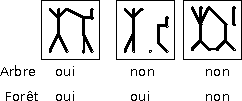
\includegraphics[width=300px]{Images/fig7.pdf} \\

\titre{Arbre couvrant :} A partir d'un graphe connexe, on peut se réduire à un arbre en "coupant" des arêtes. C'est l'arbre couvrant.

\titre{Simplification :} On suppose que les sommets sont $\{1, \ldots , n\}$ \\

\titre{Matrice d'adjacence :} \\$M = \displaystyle{(m_{ij})_{1\leq i \leq n,1\leq j \leq n}}$ où $m_{ij} = \left\{ \begin{array}{l} 1 \mathrm{si} (i,j) \in A \\ 0 \mathrm{sinon} \end{array} \right.$

\titre{Exemple : }\\
\begin{minipage}{0.4\linewidth}
$\left[\begin{array}{ccccc}
	0 & 1 & 0 & 0 & 1 \\
	0 & 0 & 0 & 1 & 0 \\
	0 & 1 & 0 & 1 & 0 \\
	0 & 0 & 0 & 0 & 0 \\
	0 & 1 & 0 & 1 & 1 \\
\end{array}\right]$
\end{minipage}
\begin{minipage}{0.4\linewidth}
\hspace{2cm} 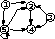
\includegraphics[width=100px]{Images/fig8.pdf}
\end{minipage}

On utilisera donc un tableau bidimensionnel. \\

\titre{Graphes par listes d'adjacences :} A chaque sommet est associée une liste qui contient les sommets qui lui sont adjacents. \\

On utilisera donc un tableau de listes.  \\

\titre{Exemple :}\\
$\begin{array}{l}
	1 : 5,2 \\
	2 : 4 \\
	3 : 2,4 \\
	4 : \\
	5 : 2,4,5 \\
\end{array}$ \newpage

\titre{Comparaison des deux représentations :} \\
\begin{tabular}{l|p{4cm}|p{4cm}}
	& Matrice & Listes \\ \hline
Espace & $O(n^2)$ & $O(n^2)$ au pire cas, $O(n)$ au meilleur cas \\ \hline
Initialisation & Pour i de 1 à n faire (Pour j de 1 à n faire) M[i,j]=0, donc $O(n^2)$ & Pour i de 1 à n faire (T[i] = liste vide), donc $O(n)$ \\ \hline
Test d'adjacence & $O(1)$ & $O(n)$ au pire cas, $O(\mathrm{nbVois})$ au cas moyen, $O(1)$ au meilleur cas \\ \hline
Afficher les voisins & $O(n)$ & $O(n)$ au pire cas, $O(\mathrm{nbVois})$ au cas moyen, $O(1)$ au meilleur cas \\ \hline
Ajouter l'arête $(u,v)$ & T[$u$].insererEnTete($v$) $O(1)$ & M[u,v] = 1 $O(1)$ \\ \hline
\end{tabular} \\

\titre{Conclusion :} 
\begin{itemize}
	\item Si on a un grand graphe avec peu d'arêtes par rapport au nombre de sommets (ou alors vraiment beaucoup, dans ce cas on peut inverser), la représentation en listes est préférable.
	\item Si on a un petit graphe, une matrice est plus simple à manipuler et pas plus couteuse
	\item Pour les autres cas, le choix dépendra du contexte.
\end{itemize}
